
\medskip

\emph{Les deux parties A et B sont indépendantes.}

\medskip

\textbf{Partie A : absorption du principe actif d'un médicament}

\smallskip

Lorsqu'on absorbe un médicament, que ce soit par voie orale ou non, la quantité de principe actif de ce médicament dans le sang évolue en fonction du temps. Cette quantité se mesure en milligrammes par litre de sang.

\smallskip

Le graphique ci-dessous représente la quantité de principe actif d'un médicament dans le sang, en fonction du temps écoulé, depuis la prise de ce médicament.

\smallskip

%\hspace{-1.1cm}
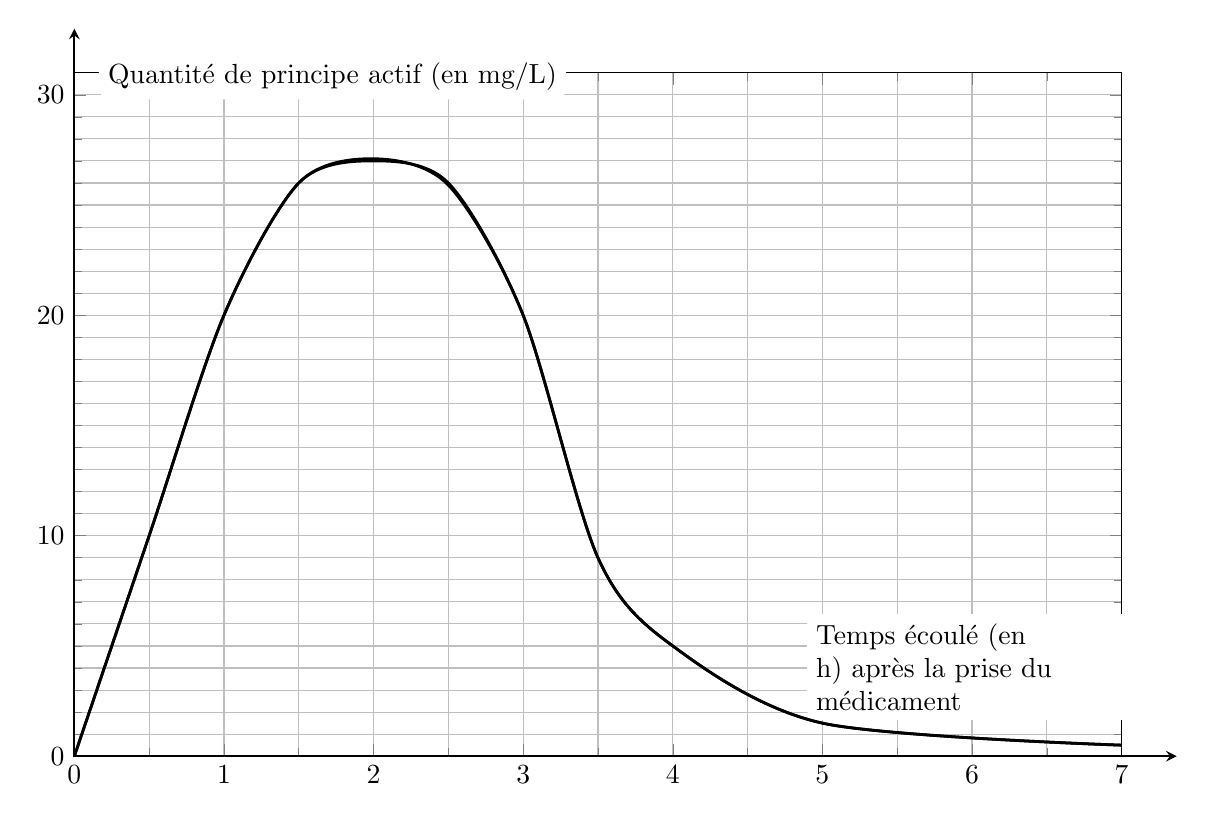
\begin{tikzpicture}[x=2cm,y=2.8mm,>=stealth]

\begin{axis}[
x=1.9cm,y=2.8mm,
xmin=0, xmax=7.,
ymin=0, ymax=31,
xtick={0,1,...,7}, ytick={0,10,20,30},
minor xtick={0,0.5,...,7}, minor ytick={0,1,...,31},
xmajorgrids=true, ymajorgrids=true,
xminorgrids=true, yminorgrids=true]
\addplot[line width=1pt,smooth]
coordinates {
	(0,0)(0.5,10)(1,20)(1.5,26)(2,27)(2.5,26)(3,20)(3.5,9)(4,5)(5,1.5)(7,0.5)
};
\addplot[line width=1pt,smooth]
coordinates {
	(0,0)(0.5,10)(1,20)(1.5,26)(2,27.1)(2.5,25.9)(3,20)(3.5,9)(4,5)(5,1.5)(7,0.5)
};
\end{axis}	

\draw [line width=0.7pt,<->] (0,33) node[fill=white, rounded corners,below right=3mm] {Quantité de principe actif (en mg/L)}--(0,0)--(7,0) node[above left=4.5mm, text width=4 cm,fill=white,rounded corners] {Temps écoulé (en h) après la prise du médicament};
\end{tikzpicture}

\begin{enumerate}
	\item  Quelle est la quantité de principe actif dans le sang, trente minutes après la prise de ce médicament ?
	
	\item Combien de temps après la prise de ce médicament, la quantité de principe actif est-elle la plus élevée ?
\end{enumerate}

\textbf{Partie B : comparaison de masses d'alcool dans deux boissons}

\smallskip

On fournit les données suivantes :

\smallskip

\begin{tabularx}{\linewidth}{|X|X|} \hline
	\rule{0pt}{14pt}\textbf{Formule permettant de calculer la masse d'alcool en g dans une boisson alcoolisée :}

$$m = V \times d \times 7,9$$
	
$ V $: volume de la boisson alcoolisée en cL
	
\smallskip
	
$ d $: degré d'alcool de la boisson
	
(exemple, un degré d'alcool de 2\,\% signifie que $d$ est égal à 0,02)\rule[-2mm]{0pt}{1mm}
&\textbf{Deux exemples de boissons alcoolisées :}	
\medskip
		
\begin{tabular}{c|c}
\textbf{Boisson} \tikz[baseline ={(a.base)}]{\node (a) at(0,0)[circle, draw]{\textbf{1}};} &\textbf{Boisson} \tikz[baseline ={(a.base)}]{\node (a) at(0,0)[circle, draw]{\textbf{2}};}\\[8pt]
Degré d'alcool : 5\,\%& Degré d'alcool : 12\,\% \\ [8pt]
Contenance : 33 cL&Contenance 125 mL \\[8pt]
\end{tabular}\\ \hline	
\end{tabularx}

\smallskip

\textbf{Question :} la boisson \tikz[baseline ={(a.base)}]{\node (a) at(0,0)[circle, draw]{\textbf{1}};} contient-elle une masse d'alcool supérieure à celle de la boisson \tikz[baseline ={(a.base)}]{\node (a) at(0,0)[circle, draw]{\textbf{2}};} ?


